
Since this has been practically derived earlier in this document, the definition of the principle is given below for reference.

{\itshape Definition}: {\bfseries Principle of Conservation of Momentum}: "If the net external forces $\vec{F}_{ext}$ on an $N$-particle system is zero, the systems total mechanical momentum $\vec{P} = \sum_{n=1}^{N} m_i v_i$."

% ------- EXAMPLE: PERFECTLY INELASTIC COLLISION
{\exbegin Example 2.4: Perfectly Inelastic Collision}

\begin{figure}[h]
    \centering
    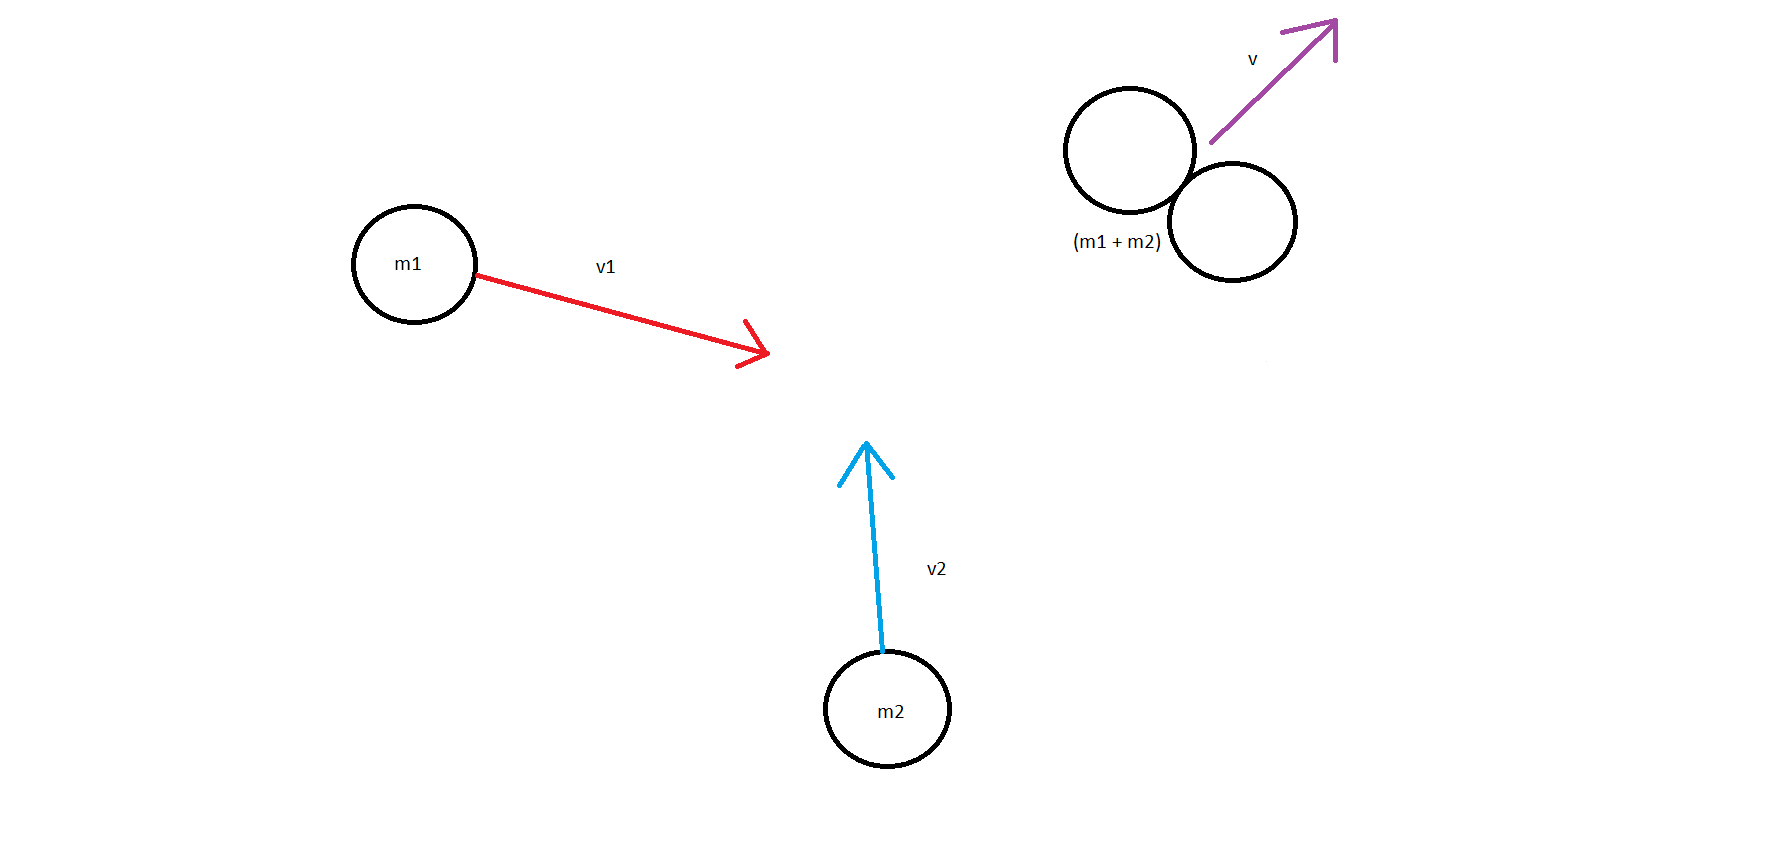
\includegraphics[width=10cm]{Classical_Mechanics/2.4-momentum/ex-inelastic-coll.png}
    \caption{A perfectly inelastic collision with no external forces conserving the systems momentum.}
    \label{fig:ex-inelastic-coll}
\end{figure}

Two bodies, $m_1$ and $m_2$, are moving at speeds $v_1$ and $v_2$, respectively. They collide and lock together as shown in figure \ref{fig:ex-inelastic-coll}. Given there are no external forces on these masses, the initial momentum, $\vec{P}_i$, is given as:

\begin{equation}
    \vec{P}_i = m_1 \vec{v}_1 + m_2 \vec{v}_2
    \label{eqn:ex2-4-inelastic-collision-i}
\end{equation}

\noindent and the final total mechanical momentum, $\vec{P}_f$, is:

\begin{equation}
    \vec{P}_f = (m_1 + m_2) \vec{v}.
    \label{eqn:ex2-4-inelastic-collision-f}
\end{equation}

Setting equations \ref{eqn:ex2-4-inelastic-collision-i} and \ref{eqn:ex2-4-inelastic-collision-f} equal to each other because the momentum is conserved (no external forces), we find,

\begin{equation*}
    \vec{P}_i = \vec{P}_f \rightarrow m_1 \vec{v}_1 + m_2 \vec{v}_2 = (m_1 + m_2)\vec{v}
\end{equation*}

\noindent and solving for $\vec{v}$, we find $\vec{v} = \frac{m_1 \vec{v}_1 + m_2 \vec{v}_2}{m_1 + m2}$.

A special case for this example is when one of the masses is initially at rest ($\vec{v}_2 = 0$). This yields the result:

\begin{equation*}
    \vec{v} = \frac{m_1}{m_1 + m_2}\vec{v}_1.
\end{equation*}

\noindent where $\vec{v}$ is in the same direction as $\vec{v}_1$ but the speed is reduced by the preceding mass ratio.

{\exend}

Note on the usage of the conservation of momentum.
This principle is the backbone of rocket propulsion. The rocket uses its fuel to push towards the launchpad in order to boost the rocket and payload into the air. The trick is to use Newton's third law of reactions. However, as the rockets gets further up, the fuel (some extra mass) is being depleted over time. This causes a tricky situation. The desire is to have the least amount of mass as possible so some rockets are boosted in stages, dumping large rocket engines off to make the rocket and payload lighter.
